\documentclass{report}
\usepackage{charter}
\usepackage{listings}
\usepackage[showframe=false, a4paper, margin=3.5cm]{geometry}
\usepackage{graphicx}
\usepackage{FiraSans}
%\usepackage{FiraMono}

\usepackage{hyperref}

\newtheorem{observation}{Observation}
\newtheorem{exercise}[observation]{Exercise}

\begin{document}
\title{Yampa}
\author{Richard J.\ Lupton}
\lstset{language=Haskell, captionpos=b, basicstyle=\footnotesize\ttfamily, keywordstyle=\bfseries, commentstyle=\itshape, breaklines=true}
\linespread{1.45}

\newcommand{\hask}[1]{\texttt{#1}}
\newcommand{\yampaMain}{{\hask{yampaMain}} }

\maketitle

\chapter{What is Yampa?}
Yampa is a Haskell library for functional reactive programming. Functional reactive programming is a high-level declarative style of programming for systems which must respond to continuous streams of input, which are often time dependant, without undue delay. Example of such systems include video games, robots, animations and simulations. Haskell with its lazy evaluation, and separation of pure and impure code doesn't make it obvious how to work in these kinds of domains, without adopting a procedural style, so Yampa was developed to provide a more idiomatic approach.

\section{How does Yampa operate?}

Functional Reactive Programming is about processing signals. At its core, Yampa takes a varying input signal (in applications this might be, for example, the temperature from a temperature sensor), and processes it in some way, providing a corresponding varying output signal on the other side (continuing our imaginary example, this might include information on whether a heater should be on or not). The upper part of Figure \ref{fig:overview} illustrates this idea.

So Yampa is concerned with building objects which can take a continuously varying input and provide a corresponding continuously varying output. If we refer to values which continuously vary as \emph{signals}, then Yampa is a library concerned with building and using \emph{signal functions}.

The bulk of Yampa is concerned with building signal functions. However, it is useful to see how a signal function is actually used in real world Haskell code to process signals. The tool that integrates signal functions into normal Haskell code is called \hask{reactimate}. \hask{reactimate} is a sample-process-output loop. The bottom part of Figure \ref{fig:overview} illustrates an idealised loop. \hask{reactimate} has three important inputs.

First \hask{reactimate} has an input of type \hask{IO a}, whose role is to take a sample of a signal which takes values of type \hask{a}. It might get the position of a mouse cursor, determine whether a key on the keyboard has been pressed, or get the temperature from a temperature sensor. Secondly, \hask{reactimate} needs a signal function, which is described using Yampa code. After collecting its input sample, of type \hask{a}, \hask{reactimate} processes it with the signal function and obtains an output sample, of type \hask{b}, say. \hask{reactimate} then has an output action, which knows what to do with this value of type \hask{b} in the outside world. For example, our output sample might be a set of coordinates to position an image on the screen, and our output function will take these coordinates and render the image there. The output \hask{IO} action comes back with a value of type \hask{Bool}, which encodes whether reactimate should continue looping or stop. So the input to \hask{reactimate} which describes how our signal should be output to the word is of type \hask{b -> IO Bool}.

Clearly, \hask{reactimate} should be capable of input and output, and so it should be a function in the \hask{IO} monad, and indeed, \hask{reactimate} returns a value of type \hask{IO ()}. In addition, \hask{reactimate} should receive some initialisation information, again of type \hask{IO a}.

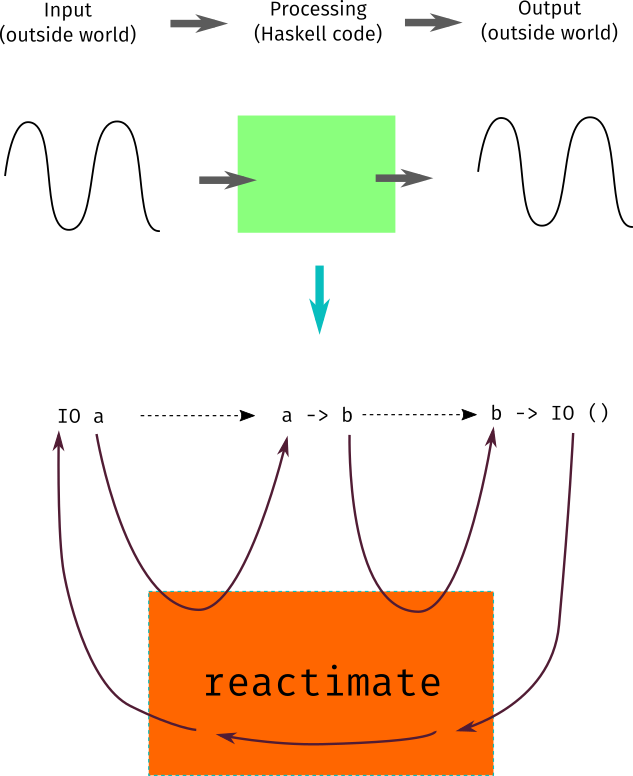
\includegraphics[height=300pt]{Diagrams/overview.png}

So \hask{reactimate} continuously samples the input, processes it with a signal function, and performs some output, until our output function says to stop. The above captures the essence of what reactimate does, but in reality the type of reactimate is a little more opaque:

\begin{lstlisting}
reactimate :: IO a
    -> (Bool -> IO (DTime, Maybe a))
    -> (Bool -> b -> IO Bool)
    -> SF a b
    -> IO ()
\end{lstlisting}

The first \hask{IO a} here is the initialisation input, and the value of type \hask{a} is the value of the first sample. The second input, of type \hask{Bool -> IO (DTime, Maybe a)} is our input function. In the definition of \hask{reactimate} the input value of \hask{Bool} is unused, so really one just needs to specify a value of type \hask{IO (DTime, Maybe a)}. In fact to make this simpler, lets define

\begin{lstlisting}
sInput :: IO (DTime, Maybe a) -> Bool -> IO (DTime, Maybe a)
sInput inp _ = inp
\end{lstlisting}

\noindent to convert a value of type \hask{IO (DTime, Maybe a)} in a value of type \hask{Bool -> IO (DTime, Maybe a)}. Now lets examine the values wrapped in the \hask{IO} type. First \hask{DTime}: \hask{reactimate} doesn't have a built in time tracking system, so on each sample of the input signal, one is required to input the elapsed time since the last sample was taken. \hask{DTime} is a synonym for \hask{Double} used to represent this. Later, we define our own reactimate which should work on any POSIX system, and hides this time tracking. Presumably it is kept visible for systems with less uniform or custom time tracking requirements. The second value here, of type \hask{Maybe a}, is the input sample, wrapped in \hask{Maybe} since there may be no input signal, or our sampling may fail. If a value of \hask{Nothing} is fed in, then the value from the previous sample is used.

The third input to \hask{reactimate} specifies how to deal with output. Again, the first \hask{Bool} in \hask{(Bool -> b -> IO Bool)} is unused, so lets define

\begin{lstlisting}
sOutput :: (b -> IO Bool) -> Bool -> b -> IO Bool
sOutput out _ = out
\end{lstlisting}

\noindent to wrap a value of type \hask{b -> IO Bool} in the type required for \hask{reactimate}. The value of type \hask{b -> IO Bool} works as described above, where a value of \hask{True} from the output function indicates to \hask{reactimate} that it should stop. The fourth value of type \hask{SF a b} is the signal function, processing a signal taking values of type \hask{a} into a signal taking values of type \hask{b}. Yampa is concerned with building these signal functions. This will be the subject of (most of) the remainder of this guide.

Using our simplified input and output wrappers, we define a simplified version of \hask{reactimate}:

\begin{lstlisting}
sReactimate :: IO a -> IO (DTime, Maybe a) -> (b -> IO Bool) -> SF a b -> IO ()
sReactimate init inp out sigFun = reactimate init (sInput inp) (sOutput out) sigFun
\end{lstlisting}

\noindent which looks a little clearer, and more like what we discussed above. In fact, we will define a function \yampaMain

\begin{lstlisting}
yampaMain :: IO a -> IO (Maybe a) -> (b -> IO Bool) -> SF a b -> IO ()
\end{lstlisting}

\noindent which also deals with the timing in POSIX compatible systems. We write this in a module \hask{YampaUtils.hs} which we will use in the rest of this guide. Listing \ref{lst:yampaUtils} gives the complete contents of the module. Note \yampaMain is essentially the same as \hask{sReactimate} but wrapped in a time tracking system.

\lstinputlisting[caption={YampaUtils.hs}, frame=single, label=lst:yampaUtils]{./src/YampaUtils.hs}

\section{The structure of a Yampa program}

One can think of Yampa programs as programs of the form illustrated in Listing \ref{lst:generalForm}. To write a Yampa program, we need to specify an initialization, input and an output function, and also construct a signal function to do the required transformations. We then feed all this in to \yampaMain which does the processing we require.

\begin{lstlisting}[caption={General form of a Yampa program}, label={lst:generalForm}]
import FRP.Yampa as Y
import YampaUtils

init :: IO a
-- Do some initialisation

input :: IO (Maybe a)
-- Get some input

output :: b -> IO Bool
-- Do some output

sigFun :: SF a b
-- Do some signal transformations

main :: IO ()
main = yampaMain init input output sigFun
\end{lstlisting}

Of course, real programs will take many different forms, but the idealised above form illustrates what we need to build in order to have an executable program.

\section{Signals and signal functions}

Yampa is a library for building and using signal functions. We have deliberately avoided making precise what is meant by a signal for two reasons

One can think of a signal taking values of type \hask{a}, or more succintly a signal of type \hask{a}, as a value of type \hask{a} with a context. Indeed, one can really think of it as being a value of type \hask{IO a} (see for instance \hask{getPOSIXTime} and compare it with the output from the \hask{time} signal function later). Like any other value of type \hask{IO a}, extracting values at different times can yield different results.


\chapter{Hello, Yampa}
Now we've pinned down the mechanics of how we will incorporate our signal functions into real working code, we can write our first example. Save a copy of \hask{YampaUtils.hs} in your working directory, for your use in these examples. Our first example, Listing \ref{lst:helloYampa}, is the Hello, World of Yampa.

\lstinputlisting[caption={HelloYampa.hs}, label=lst:helloYampa]{./src/HelloYampa.hs}

Our discussion in the introduction about \hask{reactimate}, and our tidied version \yampaMain, should give you a rough idea of what is going on here. \yampaMain first calls \hask{initialise}, which prints some text to the screen, but provides no input (or, more precisely, provides as input \hask{()}). The input function passed to \yampaMain is just \hask{return Nothing}, which again provides no input to the system.

\hask{waitTwo} is a signal function, and is the new code in this listing. For the moment, lets just observe that it converts a signal of values of type \hask{()} into a signal of values of type \hask{Bool}, which is what its type signature \hask{SF () Bool} is meant to indicate (`` a signal function from signals of type \hask{()} to signals of type \hask{Bool}'').

The output function, \hask{output}, takes this boolean value, and if its false, just instructs \yampaMain to continue by passing out a \hask{False} value in the \hask{IO} monad. However, if the boolean value is true, the output function first prints a message to the screen, and then returns an \hask{IO} value of \hask{True}, which instructs \yampaMain to stop executing, and the program finishes.

Precisely when the value \hask{True} emerges from \yampaMain is determined in the signal function \hask{waitTwo}. So lets take a look at this object.

\begin{lstlisting}
waitTwo :: SF () Bool
waitTwo = time >>> arr (>=2)
\end{lstlisting}

The specification for \hask{waitTwo} is that it should take the input signal (which here is constantly taking value \hask{()}), and if \hask{waitTwo} has been transforming input values for less than 2 seconds, it should transform the input into a value \hask{False}, and otherwise, it should transform the input signal into a value \hask{True}. This boils down to saying, \yampaMain should receive a value \hask{True} to give to \hask{output}, precisely when \yampaMain has been running for 2 seconds. Compiling and running this code seems to confirm this.

So how has \hask{waitTwo} been defined? It consists of two parts combined together with the operator \hask{>>>}. First lets take a look at \hask{time}.

\begin{lstlisting}
time :: SF a Time
\end{lstlisting}

\noindent \hask{time} takes a signal of any value, and replaces it with a value of type \hask{Time}, a synonym for \hask{Double}. The value is the time the particular instantiation of \hask{time} has been in use, starting from $0$. So in our case, it takes the value \hask{()}, and replaces it with the time that \yampaMain has been using \hask{waitTwo}, which is the length of time \yampaMain has been running.

Secondly, we have \hask{arr (>=2)}. Now inspecting the type of this in ghci reveals \hask{arr} is a function which makes use of the \hask{Arrow} type class. \hask{SF} is an instance of this type class, and specialising its type signature to \hask{SF}, we have:

\begin{lstlisting}
arr :: (a -> b) -> SF a b 
\end{lstlisting}

\noindent \hask{arr} is a way of lifting pure functions into \hask{SF}, analogous to how \hask{return} lifts values in a monad, and \hask{pure} lifts values for applicative functors. More precisely, if \hask{f :: a -> b}, then \hask{arr f} takes a signal of values of type \hask{a}, and transforms it into a signal of values of type \hask{b}, by applying \hask{f} to each value of type \hask{a}. In some sense, it is the continuous signal analogue of \hask{fmap} for the functor typeclass.

In our example, we have the signal function \hask{arr (>=2)}, which by specialising to types \hask{SF} again has type:

\begin{lstlisting}
arr (>=2) :: (Num a, Ord a) => SF a Bool
\end{lstlisting}

\noindent \hask{arr (>=2)} takes a signal with numerical and orderable values, and applies \hask{(>=2)} to these values. So our transformed signal will output \hask{True} precisely when the input signal takes on values greater than or equal to 2.

So we have two signal functions, with an operator which combines them (a \emph{combinator}). Lets inspect the type of \hask{>>>}, specialised to \hask{SF} again.

\begin{lstlisting}
(>>>) :: SF a b -> SF b c -> SF a c
\end{lstlisting}

\noindent The type signature (and the fact that the more general version is for objects from the typeclass \hask{Category}), is a giveaway for what \hask{(>>>)} does. \hask{(>>>)} is the \hask{SF} analogue of composition. Given a way of transforming signals of value type \hask{a} into signals of value type \hask{b}, and a way of transforming signals of value type \hask{b} into signals of value type \hask{c}, by performing each transformation in order, I can transform signals of value type \hask{a} into signals of value type \hask{c}. This is the function of the \hask{(>>>)} combinator. More precisely, \hask{f >>> g} first transforms with \hask{f}, and then with \hask{g} (recall \hask{f.g} first applies g \emph{then} applies \hask{f}).

So now we can analyse what \hask{waitTwo} actually does. \hask{waitTwo} takes an input signal of values \hask{()}, and replaces these values with the time which \yampaMain has been running. It then takes this time, and if it is less than 2 seconds, replaces this time value with a \hask{False}. Otherwise, it replaces this time value with \hask{True}. In total, \hask{waitTwo} transforms \hask{()} into \hask{False} if \yampaMain has been running less than 2 seconds, and \hask{True} once its been running at least two seconds.

\begin{observation}
Observe that \hask{arr (f.g) = arr g >>> arr f}. Observe that \hask{time} is not the \hask{arr} of a pure function.
\end{observation}

\section{Building signal functions}

Our first example is intentionally not the most intricate or complicated of examples. We build a very simple signal function, with the intention of showing how a Yampa program fits together.

The bulk of the Yampa library is concerned with building signal functions. Rather than building signal functions explicitly, Yampa supplies a basic set of signal functions (we saw for instance, \hask{time}, above), and a set of \emph{combinators} for combining various signal functions (for instance, signal function composition \hask{>>>}).

\section{Some basic signal functions and combinators}

Lets begin with some of the basic signal functions which Yampa provides. As one might expect from a library based around transformations, one has analogues for the identity map, and constant maps.

\begin{lstlisting}
identity :: SF a a
constant :: b -> SF a b
\end{lstlisting}

\noindent Of course, \hask{identity} preserves the value of a signal, and \hask{constant v} takes a signal, and replaces its value by the value \hask{v}.

\begin{exercise}
Write definitions for \hask{identity} and \hask{constant} in terms of \hask{arr}.
\end{exercise}

In our first example, we saw the signal function \hask{time}. \hask{time} takes a signals value, and replaces it with the \emph{local} time, that is the time a signal function has been processing a signal. For the moment, this would appear to be the same time as \yampaMain has been running, and with what has been covered so far, it is, but later we will see that signal functions can be switched in and out in response to events, at which point the time counter starts over from zero. For the sake of completeness (recall \hask{Time} is a synonym for Double):

\begin{lstlisting}
time :: SF a Time
\end{lstlisting}

An interesting built in function is \hask{integral}. This performs numerical integratation of a signal over time. Of course this is useful for describing dynamical systems!

\begin{lstlisting}
integral :: SF Double Double
\end{lstlisting}

\hask{integral} actually has a more general type than the above, but this suffices for now. Yampa provides an similar signal function for derivatives also.

\begin{observation}
\hask{time = constant 1.0 >>> integral}.
\end{observation}

We also have, as we have seen already, a way of lifting pure functions \hask{a -> b} to values of type \hask{SF a b}:

\begin{lstlisting}
arr :: (a -> b) -> SF a b
\end{lstlisting}

\noindent \hask{arr f} will take a signal of type \hask{a}, and process its value with \hask{f}, to create a signal of type \hask{b}.

Now that we have a basic collection of arrows, we woud like some ways to combine them, to form more interesting arrows. The type constructor \hask{SF} is an instance of the \hask{Arrow} typeclass, a generalisation of the \hask{Monad} type class, so we have all the combinators from \hask{Arrow} available for use. We have already seen \hask{arr} above, which is part of the \hask{Arrow} interface, and earlier we saw \hask{(>>>)}.

\hask{(>>>)} is the composition operator for signal functions. \hask{(f >>> g)} applies \hask{f} to a signal, then \hask{g} (note the order is reverse of \hask{.}). Similarly, \hask{(<<<)} is the composition operator the other way around, so \hask{(f <<< g)} performs \hask{g} then \hask{f}.

\begin{lstlisting}
(>>>) :: SF a b -> SF b c -> SF a c
(<<<) :: SF b c -> SF a b -> SF a c
\end{lstlisting}

Sometimes we want to process a signal in two different ways. The combinator \hask{(\&\&\&)} is designed to allow us to do exactly that.

\begin{lstlisting}
(&&&) :: SF a b -> SF a c -> SF a (b,c)
\end{lstlisting}

\noindent Here \hask{(f \&\&\& g)} is intended to mean take the value of a signal, and apply \hask{f} to it, placing the output in the first component of a tuple. Also apply \hask{g} to the value of the signal, and place the output in the second component of the tuple.

Since we can produce a signal which takes a tuple for values, (which we can think of as being two signals captured in one), we have combinators for processing them.

First we have \hask{(***)}, which allows us to take two signal functions and make each act on a particular element of a tuple.

\begin{lstlisting}
(***) :: SF a1 b1 -> SF a2 b2 -> SF (a1, a2) (b1, b2)
\end{lstlisting}

\noindent \hask{(f *** g)} acts on a signal which takes a tuple for values, by applying \hask{f} to the first component, and \hask{g} to the second component.

Sometimes, we only want to transform one of the elements of a signal of tuple type. While something of the form \hask{(f *** identity)} would do, Yampa defines such combinators for us:

\begin{lstlisting}
first :: SF a b -> SF (a, c) (b, c)
second :: SF b c -> SF (a, b) (a, c)
\end{lstlisting}

\noindent \hask{first f} transforms only the first component of a signal of tuple values with \hask{f}, and \hask{second g} transforms only the second component of a signal with tuple values with \hask{g}.

\begin{exercise}
Write \hask{second} in terms of \hask{first} and \hask{arr}.
\end{exercise}

\begin{observation}
\hask{ (f *** g) = (first f) >>> (second g) }.
\end{observation}

Our last combinator is \hask{loop}. \hask{loop} allows us to build recursive signal functions. It has type

\begin{lstlisting}
loop :: SF (a, c) (b, c) -> SF a b
\end{lstlisting}

\noindent \hask{(loop f)} is obtained from \hask{f} by looping its values' second component back in to \hask{f} for the next sample.

\section{Arrow notation}

The above primitives and combinators allow us to form more complex signal functions. In fact, any combination of basic signal functions can be formed. However, using the combinators directly can often lead to code which is difficult to read. For this reason, the arrow syntax was developed. This is the arrow analogue of monadic do notation. It allows us to express more clearly how we wish to process the values which signals take. A preprocessor transforms this notation into a description using the combinators we described above. When using arrow notation in ghci, load ghci with the -XArrows option, e.g. \hask{ghci -XArrows}. Similarly, when compiling with ghc, use the -XArrows option, e.g. \hask{ghc -XArrows main.hs}.

Let us first inspect the general form of a block in arrow syntax. Also, take a look at the example that follows the discussion, since this will make it clearer. The basic form of arrow syntax is given in the following.

\begin{lstlisting}
sigFun :: SF a b
sigFun = proc input -> do
  processedSample1 <- sigFun1 -< sample1
  processedSample2 <- sigFun2 -< sample2
  ...
  returnA -< finalSample
\end{lstlisting}

\hask{proc} is a keyword to indicate that the following is a block written in arrow syntax. \hask{input} represents a sample of type \hask{a}, and can be pattern matched against. A line of the form

\begin{lstlisting}
processedSample <- sigFun -< sample
\end{lstlisting}

\noindent takes the sample (from a signal) named \hask{sample}, processes it with \hask{sigFun}, and binds the resulting value to \hask{processedSample}. We can pattern match in the position of \hask{processedSample}. The line

\begin{lstlisting}
returnA -< finalSample
\end{lstlisting}

\noindent yields \hask{finalSample} as the final transformed sample. Note there is no binding, just like (and for the same reason as) a monadic \hask{do} block. As with \hask{do} blocks, \hask{let} bindings are also allowed in arrow syntax. As a word of warning, recursive definitions in arrow syntax must be preceeded by the keyword \hask{rec}. We will investigate this fully later.

By way of example, lets describe a signal function which receives a signal of type \hask{Double}, which is intended to represent the acceleration of an object, and is intended to output a signal describing its position (assuming it starts at $0$, lets say). Using the normal combinators we could write the following:

\begin{lstlisting}
accToPos :: SF Double Double
accToPos = integral >>> integral
\end{lstlisting}

\noindent which to be fair, is clear enough. In arrow syntax however, we can write this as

\begin{lstlisting}
accToPos :: SF Double Double
accToPos = proc acc -> do
  vel <- integral -< acc
  pos <- integral -< vel
  returnA -< pos
\end{lstlisting}

\noindent So we obtain \hask{vel} (velocity) by integrating the input \hask{acc} (acceleration), and we obtain \hask{pos} (position) by integrating the velocity \hask{vel}. \hask{pos} is the value we want, so we return that. It is not too hard to imagine signal functions where using the arrow syntax can greatly aid clarity. Observe that the wiring of samples through signal functions is represented in an intuitive manner.

The above example would potentially be used in an animation program, or a simulation of some kind. We will build these kinds of programs later, but for the moment it would be nice to have some working code. We will develop our ``Hello, Yampa!'' program a little further. Here, we start by asking the user to specify a time to delay finishing the greeting, and feed this value in to \yampaMain via the initialisation value.

\lstinputlisting[caption={askAndPause.hs}, label=lst:askingAndPausing]{./src/askAndPause.hs}


\chapter{Laboratory}
As exciting as variations of ``Hello, World'' are, it would be nice to be able to create some more sophisticated examples which illustrate some of the power and expression of Yampa.

To this end, we will develop a small system which we will develop in a variety of ways.  The system will make use of Haskell's high level SDL bindings, so we can retrieve live input from the user, and also render some representation of the output signal in real-time to the screen. Make sure Haskell's high-level SDL bindings are installed on your system\footnote{The package you require is \hask{SDL}, and \emph{not} \hask{sdl2}. \hask{SDL} is the package containing the high-level bindings for SDL, while \hask{sdl2} only contains the basic wrappers for the C library. Make sure the SDL C library is installed on your operating system first (using your package manager), then for the Haskell bindings simply \hask{cabal install SDL}.}.

\lstinputlisting[caption={template.hs}, label=lst:template]{./src/template.hs}

\hask{SDLTools.hs} is a small module which wraps some common SDL tasks we will use in our programs. The code is not taxing, but its also not necessary to fully understand how each function works. The tasks they perform are largerly intuitive, and will be explained when they are used. It is listed here for completeness.

\lstinputlisting[caption={SDLTools.hs}, label=lst:SDLTools]{./src/SDLTools.hs}

% \lstinputlisting[caption={laboratory.hs}, label=lst:laboratory]{./src/laboratory.hs}


\chapter{Transforming discrete signals: Events and switching combinators}
One of the nice properties of Yampa is that it can handle continuous and discrete signals (which are realised as a type of continuous signal) in one framework. A discrete signal is thought of as a signal whose value is either ``Nothing happened'', or ``Something happened, and here is some information''. More prescisely, a discrete signal is a signal with values of type \hask{Event a} where

\begin{lstlisting}
data Event a = NoEvent | Event a
\end{lstlisting}

Examples of discrete events might be mouseclicks or key presses, or when the ambient temperature exceeds a certain level.

We refer to signals of \hask{Event} type as \emph{event streams}. A signal function of type \hask{SF a (Event b)} is called an \emph{event source}.

A sample of an event stream will take two (types of) value: either \hask{NoEvent} or \hask{Event a} for some value of type \hask{a}. However, events should not occur with infinite density on a signal, and indeed, the sampling rate provides an upper bound for how often events can occur on a signal. If this is a problem, one should implement some buffering for events.

\section{Switching and events}

Events are used to initiate changes in signal functions. Yampa provides combinators which allow us to describe switching in one signal function for another when an event occurs. The most basic of these is \hask{switch}:

\begin{lstlisting}
switch :: SF a (b, Event c) -> (c -> SF a b) -> SF a b
\end{lstlisting}

\noindent The first argument of switch is best thought of as taking the form \hask{(sigFun \&\&\& eventSource)}, where \hask{sigFun :: SF a b} and \hask{eventSource :: SF a (Event c)}. The idea is that \hask{switch} says to use the signal function \hask{sigFun}, until \hask{eventSource} supplies an event. The event will be a sample of type \hask{Event c}, and this wrapped value of type \hask{c} is used to determine what the replacement signal function should be --- this is what the second input of type \hask{c -> SF a b} does. The result is a signal function of type \hask{SF a b}.

In a more intuitive language, \hask{sigFun} is switched for a different signal function when an event occurs. Let's provide an example. We will rewrite our first hello program to use a switch to output a \hask{True} signal when a time of two seconds elapses.

\lstinputlisting[caption={HelloEvent.hs}, label=lst:helloEvent]{./src/HelloEvent.hs}

Our new version is certainly no simpler than the original, but it demonstrates basic use of events. \hask{waitTwo} is still our signal function, but now it makes use of a \hask{switch} to change its output. First \hask{waitTwo} outputs a constant signal false. When an event occurs from \hask{twoElapsed} however, it takes the value from this event (in this case \hask{()}) and uses the passed function to decide what signal function to switch to. In our case, the supplied function has a constant value \hask{constant True}, so upon an event from \hask{twoElapsed}, our signal function changes to take the value \hask{True} constantly.

So now the timing work must be done in \hask{twoElapsed}. This looks much the same as before, except now \hask{time >>> arr (>=2)} is fed into a new signal function \hask{edge}. \hask{edge} has type \hask{SF Bool (Event ())}. \hask{edge} takes an input signal of value type \hask{Bool}, and when the signal value changes (from \hask{True} to \hask{False}, or \hask{False} to \hask{True}), it ouputs an \hask{Event ()} on its output; it otherwise outputs \hask{NoEvent}. In sum then, this means an event is generated when (at least) two seconds have elapsed.

The sum effect is that our program prints its conclusion after waiting for two seconds. Notice that \hask{switch} is written in infix notation. One of the benefits of this is that it the initial signal function occurs on the left of \hask{switch} and the replacement upon an event on the right.

\begin{exercise}
When a signal function \hask{sf} is switched for a signal function \hask{sf'}, the time for \hask{sf'} starts again from zero. In other words signal functions have their own local time. Write a small program to demonstrate this.
\end{exercise}

\subsection{Other event generating functions}

We saw above how to use \hask{edge} to generate an event when a signal changes from \hask{True} to \hask{False} or \hask{False} to \hask{True}, but Yampa provides a few other functions to generate events also.

\begin{lstlisting}
never :: SF a (Event b)
\end{lstlisting}

\noindent simply never generates an event. More useful perhaps is

\begin{lstlisting}
now :: b -> SF a (Event b)
\end{lstlisting}

\noindent which generates an event (with value) of type \hask{b} immediately. In other words \hask{now v} is a signal function which has value \hask{Event v} immediately, and \hask{NoEvent} afterwards.

\begin{lstlisting}
after :: Time -> b -> SF a (Event b)
\end{lstlisting}

\noindent generates an event after some specified period time, with a value of type \hask{b}. \hask{after t v} will generate a signal of value \hask{Event v} in \hask{t} seconds, with a value of \hask{NoEvent} at all other times.

\begin{exercise}
Rewrite listing \ref{lst:helloEvent} to use \hask{after}.
\end{exercise}

\noindent For those situations where having an event reoccur at regular intervals, Yampa provides

\begin{lstlisting}
repeatedly :: Time -> b -> SF a (Event b)
\end{lstlisting}

\noindent \hask{repeatedly t v} generates a signal which has value \hask{NoEvent} at all times except whole number multiplicities of \hask{t} seconds, at which point the signal has value \hask{Event v}. Zero time is when \hask{repeatedly} starts running.

Note that \hask{edge} produces an \hask{Event ()} signal. Sometimes we might want to attach or force an event to take on certain value. This is what the function \hask{tag} is for.

\begin{lstlisting}
tag :: Event a -> b -> Event b
\end{lstlisting}

\noindent In fact since \hask{Event} is a functor (it is isomorphic to \hask{Maybe}), \hask{tag} can be defined by

\begin{lstlisting}
tag e v = fmap (const v) e.
\end{lstlisting}.


\subsection{More switches}

\subsection{Other ways of interacting with events}
Switches are the main way in which event signals interact with other signals (or discrete signals interact with continuous signals if you prefer), but there are other ways we can interact with events.



\end{document}
